Metalle lassen sich als kristalline Festkörper sehen und besitzen eine ausgezeichnete
Leitfähigkeit. Die auf dem Kristallgitter sitzenden Atome sind praktisch
ohne Ausnahme ionisiert. Elektronen die freigesetzt werden gehören deshalb nicht
mehr zu einem Atom, sondern umhüllen die Ionen. Dies hat zur Folge, dass innerhalb
des Metalls ein konstant positives Potenzial herrscht, welches um $\su{\Phi}$
vom Außenraum abweicht. Es entsteht ein Potentialtopf, wie in Abbildung \ref{topf}
dargestellt.
\begin{wrapfigure}{l}{4cm}
  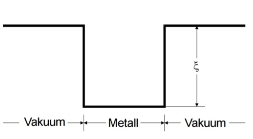
\includegraphics[width=4.3cm]{bilder/topf.jpg}
  \caption{Potentialtopfmodell im Metall \cite{504}}
  \label{topf}
\end{wrapfigure}
Tritt ein Elektron aus dem Metall aus, muss es die Potentialbarriere überwinden.
Zudem muss es die Austrittsarbeit $e_0\xi$ verrichten. Dies ist jedoch ausgeschlossen,
da Elektronen nur diskrete Energiewerte annehmen können. Spontanes verlassen ist
nur bei einer bestimmten Temperatur möglich.

Am Nullpunkt besitzen die Elektronen wegen des Pauli-Verbots eine endliche
Energie. Die Energie die maximal bei einer Temperatur von $T=0\Kel$ erreicht
werden kann, wird als Fermische Grenzenergie $\xi$ bezeichnet.

Mit der Fermi-Dirac-Verteilung
\begin{equation}
  f(E) = \frac{1}{\exp\left[\frac{E-\xi}{kT}\right]+1}
  \label{eqn:fermi}
\end{equation}
lässt sich die Wahrscheinlichkeit angeben, mit der ein Energieniveau im thermischen
Gleichgewicht besetzt ist. Der Verlauf ist in Abbildung \ref{dirac} zu sehen.
Hier wird deutlich, dass ein einzelnes Elektron eine Energie
\begin{wrapfigure}{r}{4cm}
  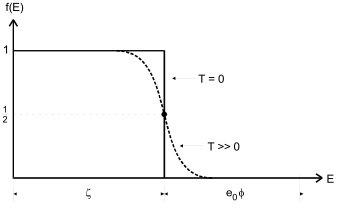
\includegraphics[width = 4cm]{bilder/dirac.jpg}
  \caption{Verlauf der Fermi-Dirac-Verteilung.\cite{504}}
  \label{dirac}
\end{wrapfigure}
\begin{equation*}
  E = \xi + e_0\su{Phi}
\end{equation*}
benötigt, um das Metall verlassen zu können. Da die Austrittsarbeit von Wolfram
für Temperaturen nahe des Schmelzpunkts groß gegenüber $kT$ ist, lässt sich mit
der Näherung
\begin{equation}
  f(E) = \exp\left[\frac{E-\xi}{kT}\right]
  \label{eqn:fermi2}
\end{equation}
gerechnet werden.

Mit der Sättigungsstromdichte $j_\su{s(T)}$ wird die Zahl der Elektonen angegeben,
die pro Zeit- und Flächeneinheit aus dem Metall austreten. Sie lässt sich mittels
Gleichung \eqref{eqn:fermi2} in Abhängigkeit der Temperatur bestimmen. Die sogenannte
Richardson-Gleichung
\begin{equation*}
  j_\su{S}(T) = 4\pi\frac{e_0 m_0 k^2}{h^3}T\exp\left[-\frac{e_0\Phi}{kT}\right]
  \label{eqn:richard}
\end{equation*}
gibt den Zzusammenhang zwischen $j_\su{S}$, $T$ und $\Phi$. Wird der Anodenstrom
gemessen, hängt dieser bei der gegebenen Apperatur nur von der Anodenspannung ab.

Ist dir Spannung zu niedrig, erreichen nicht alle Elektronen die Anode. Somit ist
eine hohe Anodenspannung nötig, damit ein unabhängiger Strom erhalten wird.
Das Ohmsche Gesetz ist aufgrund der unförmigen Bewegung der Elektronen nicht
gültig. Daher ist die Raumladungsdichte vom Ort abhängig und wird aufgrund der
steigenden Elektronengeschwindigkeit zur Anode hin kleiner. So wird das elektrische
Feld von der Kathode abgeschirmt.
Um einen Zusammenhang zwischen der Stromdichte und der Anodenspannung herzustellen
wird das Langmuir-Schottkysche Raumladungsgesetz
\begin{equation}
  j = \frac{4}{9}\epsilon_0\sqrt{\frac{2e_0}{m_0}}\frac{V^{\frac{3}{2}}}{a^2}
  \label{eqn:lang}
\end{equation}
verwendet.
Beträgt die Spannung Null, existiert entgegen \eqref{eqn:lang} ein geringer
Anodenstrom. Dieser resultiert aus der Eigengeschwindigkeit der Elektronen. Dieser
Strom wird als Anlaufstrom bezeichnet.
Mit
\begin{equation}
  j(V) = j_0\exp\left[\frac{e_0\Phi_\su{A}+e_0 V}{kT}\right] = const. \exp\left[-\frac
  {e0_v}{kT}\right]
\end{equation}
ist ein Zusammenhang zwioschen Anlaufstrom und äußerem Potential gegeben. Hierbei
ist $\Phi_\su{A}$ die Austrittsarbeit der Anode.

\begin{wrapfigure}{r}{4cm}
  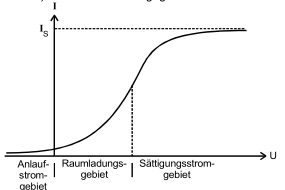
\includegraphics[width=4cm]{bilder/kennlinie.jpg}
  \caption{Kennline einer Hochvakuumdiode.\cite{504}}
  \label{kenn}
\end{wrapfigure}
Der Zusammenhang zwischen Stromdichte $j$, beziehungsweise dem Anodenstrom $I_\su{A}$,
und dem Angelegten Potential $U$ ist durch die Kennlinie einer Hochvakuumdiode
wie in Abbildung \ref{kenn} beschrieben.
Sie setzt sich aus aus dem Anlaufstromgebiet für $U<0$ sowie dem Raumladungsgebiet,
in dem die Kennlinie mit $\sqrt{U^3}$ wächst, bis sie sich asymptotisch im
Sättigungsstromgebiet einem Sättigungswert annähert.
